% Motor: XeLaTeX. Sesion 18 - material docente UTP.
% Misma estructura docente que la Sesion 17, con dos labs.
\documentclass[aspectratio=169,10pt,c]{beamer}
% Reutiliza sin cambios la identidad visual UTP validada en la Sesion 09.
% Reutiliza sin cambios la identidad visual UTP validada en la Sesion 08.
% Reutiliza sin cambios la identidad visual UTP validada en la Sesion 05.
% La segunda ruta permite compartir los assets comunes sin duplicar binarios.
\input{../../Sesion05/slides/header.tex}
\graphicspath{{../../Sesion05/slides/assets/}}



% El mapa de regiones es la captura del curso que ya esta en la Sesion 17.
\graphicspath{{assets/}{../../Sesion17/slides/assets/}{../../Sesion05/slides/assets/}}
% Bloques de código con el mismo estilo que la Sesion 11.
\usepackage{listings}
\lstset{basicstyle=\ttfamily\small,backgroundcolor=\color{utpGrisClaro},
  frame=none,aboveskip=4pt,belowskip=4pt,showstringspaces=false,
  columns=fullflexible,keepspaces=true,breaklines=true,
  xleftmargin=5pt,xrightmargin=5pt,framesep=5pt}


\title{Integración de Servicios Cloud GCP}
\subtitle{Ruta Associate Cloud Engineer: Marketplace, pila LAMP y redes VPC}
\date{Semana 09 - Sesión 18}
\author{Rel Guzman}

% Separador de tema: titulo grande, subtitulo y linea roja.
\newcommand{\separador}[2]{%
\begin{frame}[plain]
\vfill
\begin{center}
{\fontsize{29}{34}\selectfont\bfseries #1}\par
\vspace{2mm}
{\small #2}\par
\vspace{4mm}
{\color{utpRojo}\rule{8.5cm}{1.2pt}}
\end{center}
\vfill
\end{frame}}

\begin{document}

{\setbeamertemplate{footline}{}\maketitle}

% ------------------------------------------- Revision de la sesion anterior
\begin{frame}{Revisión de la sesión anterior (1/2): dos puertas}
\begin{block}{Lo que hicimos}
\small En el lab \emph{Explora la consola de Google Cloud y Cloud Shell} hiciste \textbf{lo mismo de dos maneras}: creaste un bucket con clics y otro con un comando.
\end{block}
\begin{columns}[T,onlytextwidth]
\column{.48\textwidth}
\begin{exampleblock}{La consola}
\small Una \textbf{página web} con menús y formularios. Sirve para \textbf{ver} y para hacer algo por primera vez.\par\smallskip
\emph{Se parece a:} la banca por Internet.
\end{exampleblock}
\column{.48\textwidth}
\begin{exampleblock}{Cloud Shell}
\small Una \textbf{terminal} en el navegador, ya lista. Sirve para \textbf{repetir} y automatizar.\par\smallskip
\emph{Se parece a:} dictarle el pedido al cocinero.
\end{exampleblock}
\end{columns}
\par\vspace{1mm}
\begin{alertblock}{La idea que seguimos usando hoy}
\small Las dos puertas llevan al \textbf{mismo lugar}: lo que creas con una, lo ves con la otra.
\end{alertblock}
\end{frame}

\begin{frame}{Revisión de la sesión anterior (2/2): pregunta rápida}
\begin{columns}[T,onlytextwidth]
\column{.48\textwidth}
\begin{block}{Cómo se lee un comando}
\small \texttt{gcloud storage buckets create gs://nombre}\par\smallskip
\texttt{gcloud}: el programa.\par
\texttt{storage}: el servicio.\par
\texttt{buckets}: el recurso.\par
\texttt{create}: la acción.
\end{block}
\column{.48\textwidth}
\begin{exampleblock}{Qué se conserva en Cloud Shell}
\small Los \textbf{archivos} de tu carpeta personal: sí.\par
Las \textbf{variables} de la sesión: no.
\end{exampleblock}
\begin{alertblock}{Pregunta rápida}
\small Creaste un bucket con un comando. ¿Dónde más lo puedes ver? ¿Por qué?
\end{alertblock}
\end{columns}
\end{frame}

\begin{frame}[c]
\begin{block}{Logro de la sesión}
Al finalizar, podrás explicar con tus palabras \textbf{qué es Marketplace} y para qué sirven \textbf{Jenkins} y una \textbf{pila LAMP}, \textbf{publicar una web} lista en minutos, y describir \textbf{qué es una red VPC}: sus subredes, sus direcciones IP y su firewall.
\end{block}
\end{frame}

\begin{frame}{Saberes previos}
\begin{itemize}\setlength\itemsep{10pt}
  \item Compras un celular nuevo. ¿Qué apps ya vienen instaladas? ¿Cuánto tardarías si tuvieras que instalar todo tú?
  \item En tu casa, el celular, la laptop y el televisor usan el mismo wifi. ¿Pueden ``verse'' entre ellos? ¿Y con el wifi del vecino?
  \item ¿Quién decide quién entra a un edificio? ¿Cómo lo decide?
\end{itemize}
\end{frame}

\begin{frame}[c]{Utilidad de esta sesión}
\begin{center}
\begin{minipage}{.86\textwidth}
{\large Casi todo lo que se monta en la nube necesita dos cosas: \textbf{un programa funcionando} y \textbf{una red que lo conecte}. Hoy ves las dos: primero levantas una web completa con unos pocos clics, y luego entiendes la red por donde viaja.}
\end{minipage}
\end{center}
\end{frame}

\begin{frame}{Plan de hoy: dos partes, dos labs}
\renewcommand{\arraystretch}{1.35}
\centering\small
\begin{tabular}{@{}p{1.4cm}p{6.6cm}p{4.9cm}@{}}
\toprule
\textbf{Parte} & \textbf{Qué vemos} & \textbf{Del curso}\\
\midrule
1. Teoría & Soluciones listas: Jenkins y Marketplace & \emph{Introducción al lab: Vista previa de la infraestructura}\\
\textbf{Lab 1} & Una web completa en minutos & \emph{Implementa una pila LAMP con Google Cloud Marketplace}\\
2. Teoría & Redes: VPC, subredes, IP, rutas y firewall & Módulo \emph{Redes virtuales}, desde su descripción general\\
\textbf{Lab 2} & Crear redes y probar quién habla con quién & \emph{Crea y configura redes de VPC}\\
\bottomrule
\end{tabular}
\par\vspace{3mm}
\begin{alertblock}{Cómo lo trabajamos}
\small Vamos a lo \textbf{esencial}. No vemos todos los detalles del curso: solo las ideas que necesitas para entender los dos labs.
\end{alertblock}
\end{frame}

% ------------------------------------------------ Parte 1: soluciones listas
\separador{Parte 1: soluciones listas}{\emph{Vista previa de la infraestructura}: Jenkins y Marketplace}

\begin{frame}{Una aclaración: el video dice Jenkins, el lab dice LAMP}
\begin{block}{Qué pasó}
\small El \textbf{video} de introducción se grabó hace años y muestra cómo instalar \textbf{Jenkins}. El \textbf{lab} se actualizó y hoy instala una \textbf{pila LAMP}. La idea que enseñan es \textbf{la misma}.
\end{block}
\renewcommand{\arraystretch}{1.3}
\centering\small
\begin{tabular}{@{}p{3.4cm}p{4.6cm}p{4.6cm}@{}}
\toprule
 & \textbf{En el video} & \textbf{En el lab de hoy}\\
\midrule
Qué se instala & Jenkins & Pila LAMP\\
Quién lo empaquetó & Bitnami & Google Click to Deploy\\
Nombre de la nube & GCP & Google Cloud\\
\bottomrule
\end{tabular}
\par\vspace{3mm}
\begin{exampleblock}{La idea de fondo}
\small Algo que a mano toma \textbf{horas o días}, con Marketplace toma \textbf{minutos}.
\end{exampleblock}
\end{frame}

\begin{frame}{¿Qué es Jenkins?}
\begin{columns}[T,onlytextwidth]
\column{.48\textwidth}
\begin{block}{En una frase}
\small Un programa que hace \textbf{solo} las tareas repetitivas de un equipo de programadores.
\end{block}
\begin{block}{El problema que resuelve}
\small Cada vez que alguien cambia el código, hay que \textbf{armar} el programa y \textbf{probar} que nada se rompió. A mano es lento y se olvida.
\end{block}
\column{.48\textwidth}
\begin{exampleblock}{Una comparación}
\small Un \textbf{mayordomo} que nunca duerme: apenas dejas tu trabajo sobre la mesa, él lo revisa y te avisa si algo está mal. Por eso su logo es un mayordomo.
\end{exampleblock}
\begin{alertblock}{Lo mismo, fuera de Google}
\small \textbf{GitHub Actions} y \textbf{GitLab CI} hacen lo mismo. Jenkins es \textbf{gratis} y de código abierto.
\end{alertblock}
\end{columns}
\end{frame}

\begin{frame}{Jenkins, paso a paso}
\begin{center}
\begin{tikzpicture}[font=\small,
  caja/.style={draw=utpRojo,rounded corners=4pt,minimum width=2.5cm,minimum height=1.15cm,align=center}]
  \node[caja,fill=white] (a) at (0,0) {\textbf{1. Subes}\\\footnotesize tu código};
  \node[caja,fill=utpRojo!10] (b) at (3.4,0) {\textbf{2. Arma}\\\footnotesize el programa};
  \node[caja,fill=utpRojo!20] (c) at (6.8,0) {\textbf{3. Prueba}\\\footnotesize que funcione};
  \node[caja,fill=utpRojo!32] (d) at (10.2,0) {\textbf{4. Avisa}\\\footnotesize verde o rojo};
  \draw[-latex,thick] (a) -- (b);
  \draw[-latex,thick] (b) -- (c);
  \draw[-latex,thick] (c) -- (d);
\end{tikzpicture}
\end{center}
\begin{columns}[T,onlytextwidth]
\column{.48\textwidth}
\begin{block}{Una palabra nueva}
\small \textbf{Integración continua:} juntar y probar el trabajo de todos \textbf{cada vez} que alguien sube un cambio, no una vez al mes.
\end{block}
\column{.48\textwidth}
\begin{exampleblock}{Una comparación}
\small El \textbf{control de calidad} de una fábrica: cada pieza se revisa al salir, no al final del año.
\end{exampleblock}
\end{columns}
\par\vspace{1mm}
\begin{alertblock}{Lo que necesitas recordar}
\small Jenkins es \textbf{un programa que se instala en un servidor}. Para este curso, eso basta.
\end{alertblock}
\end{frame}

\begin{frame}{Instalarlo a mano o pedirlo listo}
\begin{columns}[T,onlytextwidth]
\column{.48\textwidth}
\begin{block}{A mano: horas o días}
\small
\textbf{1.} Crear una máquina virtual.\par
\textbf{2.} Conseguirle una dirección en Internet.\par
\textbf{3.} Abrirle la puerta a las visitas web.\par
\textbf{4.} Instalar el programa y lo que necesita.\par
\textbf{5.} Crear el usuario administrador.
\end{block}
\column{.48\textwidth}
\begin{exampleblock}{Con Marketplace: minutos}
\small Eliges el producto, haces clic en \textbf{Implementar} y Google hace los cinco pasos por ti.
\end{exampleblock}
\begin{block}{Una comparación}
\small Comprar una \textbf{PC ya armada}, con Windows instalado, en vez de comprar las piezas y armarla.
\end{block}
\end{columns}
\par\vspace{1mm}
\begin{alertblock}{Una palabra nueva}
\small \textbf{Implementar} (o \emph{desplegar}): dejar un programa instalado y funcionando, listo para usarse.
\end{alertblock}
\end{frame}

\begin{frame}{Marketplace: la tienda de Google Cloud}
\begin{columns}[T,onlytextwidth]
\column{.48\textwidth}
\begin{block}{Qué es}
\small Una \textbf{tienda} dentro de la consola con programas ya preparados: WordPress, Jenkins, LAMP, bases de datos.
\end{block}
\begin{block}{Qué muestra cada producto}
\small
\textbf{Descripción:} qué instala.\par
\textbf{Quién lo preparó:} Google u otra empresa.\par
\textbf{Precio:} casi siempre, lo que cuesta la máquina virtual.
\end{block}
\column{.48\textwidth}
\begin{exampleblock}{Se parece a}
\small La \textbf{Play Store} o la \textbf{App Store}: buscas, lees la ficha e instalas.
\end{exampleblock}
\begin{alertblock}{Ojo con el precio}
\small El programa puede ser gratis, pero la \textbf{máquina donde corre se cobra} mientras esté encendida. En el lab no pagas: el proyecto es temporal.
\end{alertblock}
\end{columns}
\end{frame}

% ------------------------------------------------------------------ Lab 1
\separador{Lab 1, paso a paso}{\emph{Implementa una pila LAMP con Google Cloud Marketplace}}

\begin{frame}{¿Qué es una pila LAMP?}
\begin{block}{Dos definiciones}
\small \textbf{Pila} (\emph{stack}): varios programas que trabajan \textbf{uno sobre otro}. \textbf{LAMP}: las iniciales de los cuatro que se usan para hacer un sitio web.
\end{block}
\renewcommand{\arraystretch}{1.25}
\centering\small
\begin{tabular}{@{}p{0.9cm}p{2.6cm}p{4.2cm}p{4.9cm}@{}}
\toprule
 & \textbf{Programa} & \textbf{Qué hace} & \textbf{En un restaurante}\\
\midrule
\textbf{L} & Linux & El sistema operativo & El local\\
\textbf{A} & Apache & Atiende a quien visita la web & El mozo\\
\textbf{M} & MySQL & Guarda los datos & La despensa\\
\textbf{P} & PHP & Arma cada página & El cocinero\\
\bottomrule
\end{tabular}
\par\vspace{2mm}
\begin{columns}[T,onlytextwidth]
\column{.48\textwidth}
\begin{exampleblock}{Viene un quinto}
\small \textbf{phpMyAdmin}: una página para ver y editar la base de datos con clics.
\end{exampleblock}
\column{.48\textwidth}
\begin{alertblock}{Lo mismo, gratis en tu PC}
\small \textbf{XAMPP}. Y \textbf{WordPress}, que mueve muchísimos sitios, funciona sobre LAMP.
\end{alertblock}
\end{columns}
\end{frame}

\begin{frame}{Cómo viaja una visita por la pila}
\begin{center}
\begin{tikzpicture}[font=\small,
  caja/.style={draw=utpRojo,rounded corners=4pt,minimum width=2.5cm,minimum height=1.15cm,align=center}]
  \draw[black!50,dashed,rounded corners=6pt] (2.0,-1.0) rectangle (11.6,1.35);
  \node[anchor=north west,font=\footnotesize] at (2.1,1.3) {una máquina virtual con \textbf{Linux}};
  \node[caja,fill=white] (n) at (0,0) {\textbf{Tu navegador}};
  \node[caja,fill=utpRojo!10] (a) at (3.6,0) {\textbf{Apache}\\\footnotesize recibe};
  \node[caja,fill=utpRojo!20] (p) at (6.8,0) {\textbf{PHP}\\\footnotesize arma la página};
  \node[caja,fill=utpRojo!32] (m) at (10.0,0) {\textbf{MySQL}\\\footnotesize entrega datos};
  \draw[latex-latex,thick] (n) -- (a);
  \draw[latex-latex,thick] (a) -- (p);
  \draw[latex-latex,thick] (p) -- (m);
\end{tikzpicture}
\end{center}
\begin{columns}[T,onlytextwidth]
\column{.48\textwidth}
\begin{block}{En palabras}
\small Pides una página. \textbf{Apache} recibe el pedido, \textbf{PHP} la prepara con los datos que le da \textbf{MySQL}, y la página vuelve a tu navegador.
\end{block}
\column{.48\textwidth}
\begin{exampleblock}{En el restaurante}
\small El mozo toma el pedido, el cocinero prepara el plato con lo que saca de la despensa, y el mozo te lo trae.
\end{exampleblock}
\end{columns}
\par\vspace{1mm}
\begin{alertblock}{En este lab}
\small Los cuatro viven en \textbf{una sola} máquina virtual. Tú no instalas ninguno.
\end{alertblock}
\end{frame}

\begin{frame}{Lab 1, tarea 1: pide la pila LAMP}
\begin{columns}[T,onlytextwidth]
\column{.52\textwidth}
\begin{block}{Paso a paso}
\small
\textbf{1.} Menú de navegación $\rightarrow$ \textbf{Marketplace}.\par\smallskip
\textbf{2.} Busca \texttt{LAMP} y presiona Enter.\par\smallskip
\textbf{3.} Elige \textbf{Pila de LAMP de Google Click to Deploy}.\par\smallskip
\textbf{4.} \textbf{Comenzar}, marca los términos, \textbf{Aceptar} y luego \textbf{Implementar}.\par\smallskip
\textbf{5.} Si lo pide, \textbf{Habilitar} las APIs.\par\smallskip
\textbf{6.} \textbf{Zona:} la que indica tu lab. \textbf{Serie:} E2. \textbf{Tipo:} e2-medium.\par\smallskip
\textbf{7.} \textbf{Implementar} y espera el mensaje \emph{Se implementó lamp-1}.
\end{block}
\column{.44\textwidth}
\begin{alertblock}{El error más común}
\small Elegir \textbf{otra} pila LAMP de la lista. Hay varias: los pasos del lab solo coinciden con la de \textbf{Google Click to Deploy}.
\end{alertblock}
\begin{exampleblock}{Qué significa cada elección}
\small
\textbf{Zona:} en qué centro de datos queda.\par
\textbf{e2-medium:} el tamaño de la máquina (2 CPU y 4 GB de memoria).\par
\textbf{Habilitar una API:} encender el interruptor de ese servicio.
\end{exampleblock}
\end{columns}
\par\vspace{1mm}
\begin{block}{No olvides}
\small \textbf{Revisar mi progreso}. Si aparecen advertencias mientras se instala, el lab dice que las ignores.
\end{block}
\end{frame}

\begin{frame}{Lo que Marketplace hizo por ti}
\begin{center}
\begin{tikzpicture}[font=\small,
  pieza/.style={draw=utpRojo,rounded corners=3pt,fill=white,minimum width=2.75cm,minimum height=1.0cm,align=center}]
  \draw[utpRojo,thick,rounded corners=6pt,fill=utpRojo!6] (-1.8,-0.85) rectangle (11.4,1.45);
  \node[anchor=north west,font=\small\bfseries] at (-1.7,1.4) {Implementación \texttt{lamp-1}};
  \node[pieza] at (0,0) {\textbf{VM}\\\footnotesize\texttt{lamp-1-vm}};
  \node[pieza] at (3.2,0) {\textbf{Dirección}\\\footnotesize en Internet};
  \node[pieza] at (6.4,0) {\textbf{Firewall}\\\footnotesize deja pasar la web};
  \node[pieza] at (9.6,0) {\textbf{Programas}\\\footnotesize los de LAMP};
\end{tikzpicture}
\end{center}
\begin{columns}[T,onlytextwidth]
\column{.48\textwidth}
\begin{block}{Cuatro cosas, un clic}
\small Creó la máquina, le dio una dirección para visitarla, abrió la puerta de la web e instaló los programas. Son los \textbf{mismos pasos} que harías a mano.
\end{block}
\column{.48\textwidth}
\begin{exampleblock}{¿Y quién lo hizo?}
\small Un servicio que sigue una \textbf{receta} escrita. En el video se llama \emph{Deployment Manager}; hoy, \textbf{Infrastructure Manager}.
\end{exampleblock}
\end{columns}
\par\vspace{1mm}
\begin{alertblock}{Por qué importa}
\small Nada es magia: cada pieza la verás por separado en este curso. La red y el firewall, \textbf{hoy mismo}.
\end{alertblock}
\end{frame}

\begin{frame}{Lab 1, tarea 2: comprueba que funciona}
\begin{columns}[T,onlytextwidth]
\column{.48\textwidth}
\begin{block}{Paso a paso}
\small
\textbf{1.} Haz clic en \textbf{lamp-1-vm} $\rightarrow$ \textbf{Detalles}.\par\smallskip
\textbf{2.} Haz clic en \textbf{URL del sitio}.\par\smallskip
\textbf{3.} Se abre una pestaña con un mensaje de \textbf{felicitaciones}: Apache está atendiendo.
\end{block}
\begin{exampleblock}{¿Qué es la URL del sitio?}
\small La \textbf{dirección en Internet} de tu máquina. Cualquiera que la tenga puede visitar tu web.
\end{exampleblock}
\column{.48\textwidth}
\begin{alertblock}{Si la página no abre}
\small
\textbf{Espera 30 segundos} y vuelve a intentar: los programas tardan en arrancar.\par\smallskip
Si sale un aviso de \textbf{redirección}, haz clic en ese enlace.\par\smallskip
Si usas una \textbf{VPN} o la red de una empresa, prueba desde tu celular.
\end{alertblock}
\begin{block}{Tarea 3: repaso}
\small Listo: publicaste una web completa \textbf{sin instalar nada}.
\end{block}
\end{columns}
\end{frame}

% ------------------------------------------------------ Parte 2: redes
\separador{Parte 2: redes virtuales}{Módulo \emph{Redes virtuales}: VPC, subredes, direcciones IP, rutas y firewall}

\begin{frame}{Antes de empezar: cinco palabras de redes}
\renewcommand{\arraystretch}{1.4}
\centering\small
\begin{tabular}{@{}p{2.6cm}p{5.4cm}p{4.8cm}@{}}
\toprule
\textbf{Palabra} & \textbf{Qué es} & \textbf{Se parece a}\\
\midrule
\textbf{Red} & Computadoras conectadas entre sí & El wifi de tu casa\\
\textbf{Dirección IP} & El número que identifica a cada una & La dirección de una casa\\
\textbf{Puerto} & Un número de ``puerta'' dentro de la computadora & La ventanilla 3 del banco\\
\textbf{Protocolo} & El idioma en que conversan & Hablar en castellano o por señas\\
\textbf{Ping} & Un saludo corto para ver si la otra responde & Gritar ``¿me escuchas?''\\
\bottomrule
\end{tabular}
\par\vspace{3mm}
\begin{exampleblock}{Tres nombres que verás en el lab}
\small \textbf{SSH:} entrar a la terminal de otra máquina (puerto 22). \textbf{RDP:} ver el escritorio de una máquina Windows (puerto 3389). \textbf{ICMP:} el protocolo que usa \texttt{ping}.
\end{exampleblock}
\end{frame}

\begin{frame}{La red de Google}
\begin{columns}[c,onlytextwidth]
\column{.54\textwidth}
\centering
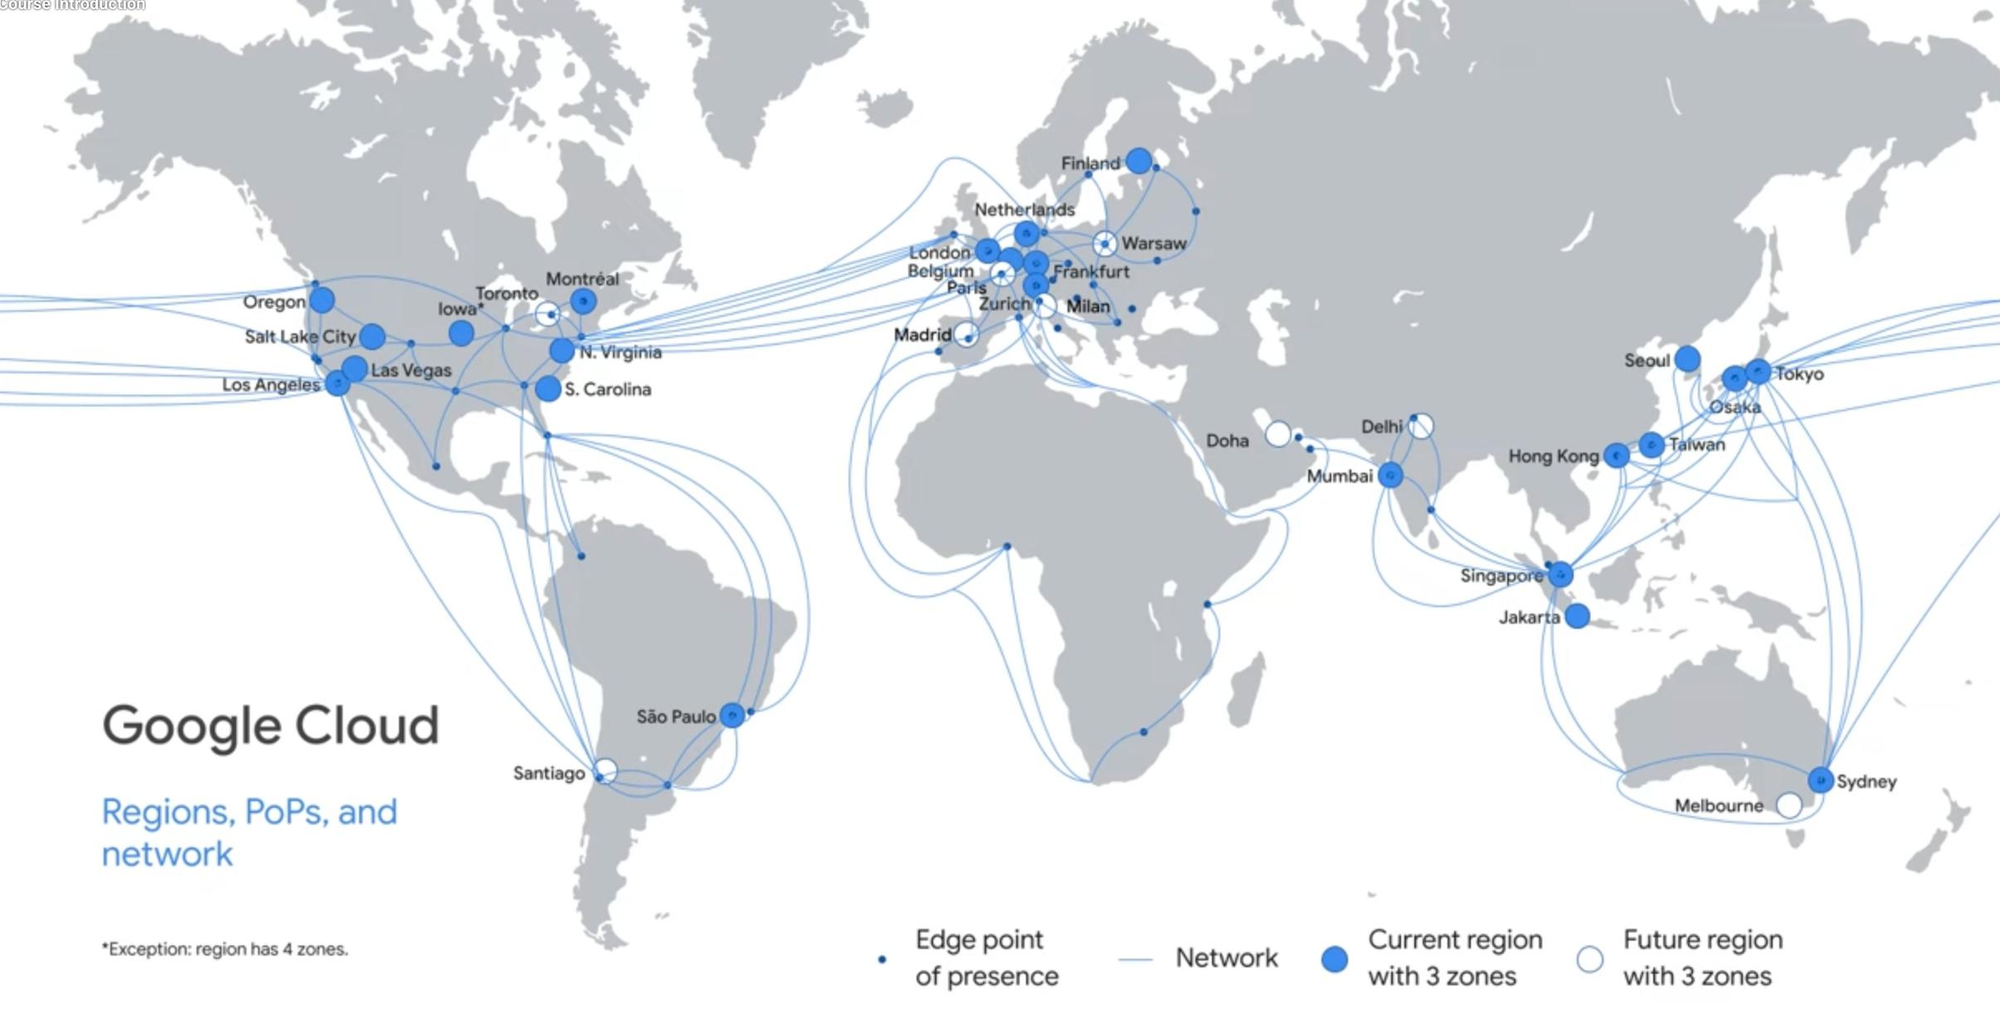
\includegraphics[width=\linewidth]{gc-mapa-regiones.png}
\par\vspace{1mm}
{\scriptsize El mismo mapa de la sesión anterior: regiones, puntos de presencia y cables.}
\column{.43\textwidth}
\begin{block}{Lo que dice el módulo}
\small Google tiene una de las redes más grandes del mundo: \textbf{fibra óptica propia}, incluso bajo el mar.
\end{block}
\begin{exampleblock}{La idea nueva}
\small Tú no tocas cables. La red se arma con \textbf{configuración}: clics o comandos.\par\smallskip
Piensa en la red como un \textbf{servicio}, no como un aparato.
\end{exampleblock}
\end{columns}
\par\vspace{1mm}
\begin{alertblock}{Una comparación}
\small Crear un \textbf{grupo de WhatsApp}: conectas a quien quieras, de cualquier país, sin tender un solo cable.
\end{alertblock}
\end{frame}

\begin{frame}{¿Qué es una VPC?}
\begin{block}{Definición}
\small \textbf{VPC} (\emph{Virtual Private Cloud}, nube privada virtual): la \textbf{red privada} de tu proyecto. Ahí se conectan tus máquinas virtuales.
\end{block}
\begin{columns}[T,onlytextwidth]
\column{.48\textwidth}
\begin{block}{El curso la describe así}
\small ``Un conjunto de \textbf{objetos} de red administrados por Google''.
\end{block}
\begin{alertblock}{Una palabra nueva: objeto}
\small \textbf{Objeto} = una ``cosa'' identificable dentro del sistema, con propiedades y configuración propias.
\end{alertblock}
\column{.48\textwidth}
\begin{exampleblock}{Los objetos de una VPC}
\small Redes, subredes, direcciones IP, rutas y reglas de firewall. Cada uno tiene \textbf{nombre} y sus propios \textbf{ajustes}.
\end{exampleblock}
\begin{block}{Una comparación}
\small Un \textbf{condominio}: es tuyo, tiene bloques, puertas numeradas, pasillos y un portero.
\end{block}
\end{columns}
\par\vspace{1mm}
\begin{exampleblock}{Lo mismo, fuera de Google}
\small En casa, tu \textbf{router wifi}. En otras nubes: \textbf{VPC} en AWS y \textbf{Virtual Network} en Azure.
\end{exampleblock}
\end{frame}

\begin{frame}{Proyecto, red y subred}
\begin{columns}[c,onlytextwidth]
\column{.54\textwidth}
\centering
\begin{tikzpicture}[font=\footnotesize]
  \draw[black!55,rounded corners=6pt] (-0.25,-0.25) rectangle (6.85,4.2);
  \node[anchor=north west,font=\small\bfseries] at (-0.15,4.15) {Proyecto};
  \draw[utpRojo,thick,rounded corners=6pt,fill=utpRojo!5] (0,0) rectangle (6.6,3.5);
  \node[anchor=north west,font=\small\bfseries] at (0.1,3.45) {Red (es mundial)};
  \draw[rounded corners=4pt,fill=white] (0.3,0.3) rectangle (3.1,2.7);
  \node[anchor=north west] at (0.35,2.65) {\textbf{Subred}};
  \node[anchor=north west] at (0.35,2.25) {región de EE.\,UU.};
  \node[draw,fill=utpRojo!20,rounded corners=2pt] at (1.05,0.9) {VM};
  \node[draw,fill=utpRojo!20,rounded corners=2pt] at (2.3,0.9) {VM};
  \draw[rounded corners=4pt,fill=white] (3.5,0.3) rectangle (6.3,2.7);
  \node[anchor=north west] at (3.55,2.65) {\textbf{Subred}};
  \node[anchor=north west] at (3.55,2.25) {región de Europa};
  \node[draw,fill=utpRojo!20,rounded corners=2pt] at (4.9,0.9) {VM};
\end{tikzpicture}
\column{.43\textwidth}
\begin{block}{De afuera hacia adentro}
\small
\textbf{Proyecto:} la caja donde vive todo.\par\smallskip
\textbf{Red:} abarca \textbf{todo el mundo}.\par\smallskip
\textbf{Subred:} un pedazo de la red en \textbf{una región}, con su propio grupo de direcciones.\par\smallskip
\textbf{VM:} vive dentro de una subred.
\end{block}
\end{columns}
\par\vspace{1mm}
\begin{columns}[T,onlytextwidth]
\column{.48\textwidth}
\begin{exampleblock}{Una comparación}
\small La red es una \textbf{empresa}; cada subred, su \textbf{oficina} en una ciudad; cada VM, un \textbf{empleado} con su anexo.
\end{exampleblock}
\column{.48\textwidth}
\begin{alertblock}{Sin red no hay VM}
\small Toda máquina virtual necesita una red. Lo comprobarás en el lab 2.
\end{alertblock}
\end{columns}
\end{frame}

\begin{frame}{Tres tipos de red}
\renewcommand{\arraystretch}{1.35}
\centering\small
\begin{tabular}{@{}>{\raggedright\arraybackslash}p{3.0cm}>{\raggedright\arraybackslash}p{5.6cm}p{4.2cm}@{}}
\toprule
\textbf{Tipo} & \textbf{Cómo son sus subredes} & \textbf{Como\ldots}\\
\midrule
\textbf{Predeterminada} (\texttt{default}) & Ya viene en cada proyecto, con una subred en cada región & el chip que ya trae el celular\\
\textbf{Modo automático} & Google crea una subred en cada región por ti & pedir el combo\\
\textbf{Modo personalizado} & Tú decides qué subredes, dónde y con qué direcciones & pedir a la carta\\
\bottomrule
\end{tabular}
\par\vspace{3mm}
\begin{columns}[T,onlytextwidth]
\column{.48\textwidth}
\begin{exampleblock}{¿Cuál conviene?}
\small \textbf{Automático:} para probar rápido.\par
\textbf{Personalizado:} para trabajos reales; tú tienes el control.
\end{exampleblock}
\column{.48\textwidth}
\begin{alertblock}{Un solo sentido}
\small De automático a personalizado \textbf{sí} se puede cambiar. De regreso, \textbf{no}.
\end{alertblock}
\end{columns}
\end{frame}

\begin{frame}{La idea más importante: ¿misma red u otra red?}
\begin{center}
\begin{tikzpicture}[font=\footnotesize,
  vm/.style={draw,fill=utpRojo!20,rounded corners=2pt,minimum width=1.0cm,minimum height=.6cm}]
  \draw[utpRojo,thick,rounded corners=6pt,fill=utpRojo!5] (0,0) rectangle (6.0,2.2);
  \node[anchor=north west,font=\small\bfseries] at (0.1,2.15) {Red 1};
  \node[vm] (a) at (1.2,0.75) {VM A};
  \node[vm] (b) at (4.8,0.75) {VM B};
  \node[anchor=north] at (1.2,0.4) {EE.\,UU.};
  \node[anchor=north] at (4.8,0.4) {Europa};
  \draw[latex-latex,thick] (a) -- node[above] {se hablan directo} (b);
  \draw[utpRojo,thick,rounded corners=6pt,fill=utpRojo!5] (7.0,0) rectangle (9.6,2.2);
  \node[anchor=north west,font=\small\bfseries] at (7.1,2.15) {Red 2};
  \node[vm] (c) at (8.3,0.75) {VM C};
  \draw[utpRojo,thick,rounded corners=6pt,fill=utpRojo!5] (10.4,0) rectangle (13.0,2.2);
  \node[anchor=north west,font=\small\bfseries] at (10.5,2.15) {Red 3};
  \node[vm] (d) at (11.7,0.75) {VM D};
  \node[anchor=north] at (10.0,0.4) {misma ciudad};
  \draw[dashed,thick] (c) -- node[above,font=\small\bfseries] {X} (d);
\end{tikzpicture}
\end{center}
\begin{columns}[T,onlytextwidth]
\column{.48\textwidth}
\begin{block}{A y B: misma red, países distintos}
\small Se hablan \textbf{directo}, por dentro, como si estuvieran en el mismo cuarto.
\end{block}
\column{.48\textwidth}
\begin{block}{C y D: redes distintas, misma ciudad}
\small \textbf{No} se hablan por dentro. Solo si cada una sale con su dirección pública.
\end{block}
\end{columns}
\par\vspace{1mm}
\begin{exampleblock}{Una comparación}
\small Dos anexos de la \textbf{misma empresa} se llaman gratis aunque estén en ciudades distintas. Dos \textbf{empresas distintas}, aunque compartan edificio, tienen que llamarse por el número público.
\end{exampleblock}
\end{frame}

\begin{frame}{El grupo de direcciones de una subred}
\begin{block}{Cómo se escribe}
\small Cada subred tiene un \textbf{rango} de direcciones, por ejemplo \texttt{10.240.0.0/20}. El número después de la barra dice \textbf{cuántas} hay: mientras \textbf{más chico}, \textbf{más direcciones}.
\end{block}
\renewcommand{\arraystretch}{1.25}
\centering\small
\begin{tabular}{@{}p{2.6cm}p{3.6cm}p{6.0cm}@{}}
\toprule
\textbf{Termina en} & \textbf{Direcciones} & \textbf{Alcanza para\ldots}\\
\midrule
\texttt{/29} & 8 & una prueba muy pequeña\\
\texttt{/24} & 256 & un salón de clases grande\\
\texttt{/20} & 4\,096 & una empresa\\
\bottomrule
\end{tabular}
\par\vspace{2mm}
\begin{columns}[T,onlytextwidth]
\column{.48\textwidth}
\begin{exampleblock}{Google se guarda 4}
\small En cada subred, \textbf{cuatro} direcciones son para que la red funcione. En una \texttt{/29} te quedan 4 para tus VMs.
\end{exampleblock}
\column{.48\textwidth}
\begin{alertblock}{¿Te quedaste corto?}
\small Se puede \textbf{agrandar} la subred sin apagar nada, como pedir más anexos en una oficina. \textbf{Achicarla}, no.
\end{alertblock}
\end{columns}
\end{frame}

\begin{frame}{Dirección IP interna y externa}
\begin{columns}[T,onlytextwidth]
\column{.48\textwidth}
\begin{block}{IP interna}
\small La tiene \textbf{toda} máquina virtual. Sirve para hablar \textbf{dentro} de su red. Google la asigna sola.
\end{block}
\begin{block}{IP externa}
\small Es \textbf{opcional}. Sirve para que te vean desde \textbf{Internet}. La \emph{URL del sitio} del lab 1 era esto.
\end{block}
\column{.48\textwidth}
\begin{exampleblock}{Una comparación}
\small La interna es tu \textbf{anexo}: solo funciona dentro de la oficina. La externa es el \textbf{número público}: cualquiera puede marcarlo.
\end{exampleblock}
\begin{alertblock}{La externa puede cambiar}
\small \textbf{Efímera:} si apagas y prendes la VM, te dan otra.\par
\textbf{Estática:} la reservas y es siempre la misma.
\end{alertblock}
\end{columns}
\par\vspace{1mm}
\begin{block}{Lo que muestra la demostración del curso}
\small Apagan una VM y la vuelven a prender: la IP \textbf{interna quedó igual}; la \textbf{externa cambió}.
\end{block}
\end{frame}

\begin{frame}{Rutas: por dónde va el tráfico}
\begin{columns}[T,onlytextwidth]
\column{.48\textwidth}
\begin{block}{Qué es una ruta}
\small Una indicación: ``para llegar a \textbf{tal destino}, ve por \textbf{aquí}''.
\end{block}
\begin{block}{Las que ya vienen}
\small
\textbf{Una por cada subred:} para que las VMs de la red se encuentren.\par\smallskip
\textbf{Una hacia Internet:} para todo lo que está afuera. Se escribe \texttt{0.0.0.0/0}, que significa ``cualquier dirección''.
\end{block}
\column{.48\textwidth}
\begin{exampleblock}{Una comparación}
\small Los \textbf{letreros de la carretera}: ``Arequipa, por la derecha''. No manejan por ti; solo indican el camino.
\end{exampleblock}
\begin{alertblock}{La ruta no basta}
\small Que exista el camino no significa que te dejen pasar. De eso se encarga el \textbf{firewall}.
\end{alertblock}
\end{columns}
\par\vspace{1mm}
\begin{block}{Para este curso}
\small No creas rutas: Google las crea y las mantiene. Solo las miras en el lab.
\end{block}
\end{frame}

\begin{frame}{Firewall: quién puede pasar}
\begin{center}
\begin{tikzpicture}[font=\small,
  caja/.style={draw=utpRojo,rounded corners=4pt,minimum width=2.6cm,minimum height=1.0cm,align=center}]
  \node[caja,fill=white] (i) at (0,0) {\textbf{Alguien}\\\footnotesize quiere entrar};
  \node[caja,fill=utpRojo!30] (f) at (5.0,0) {\textbf{Firewall}\\\footnotesize revisa su lista};
  \node[caja,fill=utpRojo!10] (v) at (10.0,0) {\textbf{Tu VM}};
  \draw[-latex,thick] (i) -- (f);
  \draw[-latex,thick] (f) -- node[above,font=\footnotesize] {si está permitido} (v);
\end{tikzpicture}
\end{center}
\begin{columns}[T,onlytextwidth]
\column{.48\textwidth}
\begin{block}{Las dos reglas que siempre están}
\small Lo que \textbf{entra}: todo \textbf{bloqueado}.\par
Lo que \textbf{sale}: todo \textbf{permitido}.\par\smallskip
Tú agregas reglas para \textbf{dejar entrar} lo que necesitas.
\end{block}
\column{.48\textwidth}
\begin{exampleblock}{Una regla dice tres cosas}
\small
\textbf{Qué:} protocolo y puerto (SSH, puerto 22).\par
\textbf{Desde dónde:} qué direcciones.\par
\textbf{A quién:} todas las VMs o solo algunas.
\end{exampleblock}
\end{columns}
\par\vspace{1mm}
\begin{alertblock}{Una comparación}
\small El \textbf{portero} del condominio con su lista de invitados: si no estás en la lista, no entras. Tú, que vives ahí, sales cuando quieres.
\end{alertblock}
\end{frame}

\begin{frame}{Precios: qué se cobra en la red}
\renewcommand{\arraystretch}{1.35}
\centering\small
\begin{tabular}{@{}p{7.4cm}p{3.6cm}@{}}
\toprule
\textbf{Tráfico} & \textbf{¿Se cobra?}\\
\midrule
Lo que \textbf{entra} a Google Cloud & No\\
Entre VMs de la \textbf{misma zona}, por su IP interna & No\\
Lo que \textbf{sale} a otra zona, a otra región o a Internet & \textbf{Sí}\\
Tener una \textbf{IP externa} & \textbf{Sí}\\
\bottomrule
\end{tabular}
\par\vspace{3mm}
\begin{columns}[T,onlytextwidth]
\column{.48\textwidth}
\begin{exampleblock}{Una comparación}
\small El teléfono de antes: \textbf{recibir} llamadas era gratis, \textbf{llamar} costaba. Y entre anexos, nada.
\end{exampleblock}
\column{.48\textwidth}
\begin{alertblock}{Dos consejos}
\small Los precios \textbf{cambian}: se consultan en la \textbf{calculadora de precios} de Google Cloud. Y una IP reservada que \textbf{no usas} cuesta más.
\end{alertblock}
\end{columns}
\end{frame}

% ------------------------------------------------------------------ Lab 2
\separador{Lab 2, paso a paso}{\emph{Crea y configura redes de VPC}}

\begin{frame}{Mapa del lab 2}
\begin{block}{De qué trata}
\small Borras la red que viene por defecto, creas \textbf{tres redes} propias y pruebas con \texttt{ping} \textbf{qué máquinas se pueden hablar}.
\end{block}
\renewcommand{\arraystretch}{1.3}
\centering\small
\begin{tabular}{@{}p{0.7cm}p{5.6cm}p{6.4cm}@{}}
\toprule
\textbf{\#} & \textbf{Tarea} & \textbf{Lo que aprendes}\\
\midrule
1 & Explora la red predeterminada & Qué trae una red, y que sin red no hay VM\\
2 & Crea una red de modo automático & Red, firewall y dos VMs; probar con \texttt{ping}\\
3 & Crea redes de modo personalizado & Lo mismo con clics y con comandos\\
4 & Explora la conectividad entre redes & Misma red: se hablan. Otra red: no\\
\bottomrule
\end{tabular}
\par\vspace{2mm}
\begin{alertblock}{Es un lab largo}
\small Tiene muchos pasos, pero se \textbf{repiten}: crear una red, una regla, una VM. La primera vez con clics; la segunda, con un comando.
\end{alertblock}
\end{frame}

\begin{frame}{Lo que tendrás al terminar}
\begin{center}
\begin{tikzpicture}[font=\footnotesize,
  vm/.style={draw,fill=utpRojo!20,rounded corners=2pt,minimum height=.55cm,inner xsep=3pt}]
  \draw[utpRojo,thick,rounded corners=6pt,fill=utpRojo!5] (0,0) rectangle (5.0,3.0);
  \node[anchor=north west,font=\small\bfseries] at (0.1,2.95) {\texttt{mynetwork}};
  \node[vm] at (2.5,1.75) {\texttt{mynet-us-vm} (EE.\,UU.)};
  \node[vm] at (2.5,0.75) {\texttt{mynet-notus-vm} (otra región)};
  \draw[utpRojo,thick,rounded corners=6pt,fill=utpRojo!5] (5.4,0) rectangle (9.5,3.0);
  \node[anchor=north west,font=\small\bfseries] at (5.5,2.95) {\texttt{managementnet}};
  \node[vm] at (7.45,1.25) {\texttt{managementnet-us-vm}};
  \draw[utpRojo,thick,rounded corners=6pt,fill=utpRojo!5] (9.9,0) rectangle (13.4,3.0);
  \node[anchor=north west,font=\small\bfseries] at (10.0,2.95) {\texttt{privatenet}};
  \node[vm] at (11.65,1.25) {\texttt{privatenet-us-vm}};
\end{tikzpicture}
\end{center}
\begin{columns}[T,onlytextwidth]
\column{.48\textwidth}
\begin{block}{Cómo leer el dibujo}
\small Tres \textbf{redes} (los marcos) y cuatro \textbf{máquinas} (las cajas). Tres máquinas están en la \textbf{misma zona}, pero en redes distintas.
\end{block}
\column{.48\textwidth}
\begin{exampleblock}{Cómo leer los nombres}
\small \texttt{us}: está en la región de EE.\,UU. \texttt{notus}: \emph{not US}, está en \textbf{otra} región. El lab te dice cuáles son.
\end{exampleblock}
\end{columns}
\par\vspace{1mm}
\begin{alertblock}{La pregunta del lab}
\small Desde \texttt{mynet-us-vm}, ¿a cuáles de las otras tres llega un \texttt{ping}?
\end{alertblock}
\end{frame}

\begin{frame}{Lab 2, tarea 1: explora la red predeterminada}
\begin{columns}[T,onlytextwidth]
\column{.48\textwidth}
\begin{block}{Primero, mira}
\small En \textbf{Red de VPC} verás lo que trae la red \texttt{default}:\par\smallskip
\textbf{Subredes:} una en cada región.\par
\textbf{Rutas:} una por subred y una hacia Internet.\par
\textbf{Firewall:} cuatro reglas que dejan entrar \texttt{ping}, SSH, RDP y lo que viene de la misma red.
\end{block}
\column{.48\textwidth}
\begin{block}{Después, borra}
\small
\textbf{1.} Borra las cuatro reglas de firewall.\par
\textbf{2.} Borra la red \texttt{default}.\par
\textbf{3.} Mira \textbf{Rutas} y \textbf{Firewall}: quedaron vacíos.
\end{block}
\begin{exampleblock}{El experimento}
\small Intenta crear una VM. Sale el error \emph{No hay más redes disponibles}. Haz clic en \textbf{Cancelar}.
\end{exampleblock}
\end{columns}
\par\vspace{1mm}
\begin{alertblock}{La lección}
\small \textbf{Sin red, no hay máquina virtual.} Es como querer un anexo en una oficina sin central telefónica.
\end{alertblock}
\end{frame}

\begin{frame}{Lab 2, tarea 2 (a): crea una red automática}
\begin{columns}[T,onlytextwidth]
\column{.50\textwidth}
\begin{block}{Paso a paso}
\small
\textbf{1.} En Cloud Shell, ejecuta el comando que da el lab para \textbf{habilitar} dos APIs.\par\smallskip
\textbf{2.} \textbf{Red de VPC} $\rightarrow$ \textbf{Crear red de VPC}. Nombre: \texttt{mynetwork}. Modo: \textbf{Automático}.\par\smallskip
\textbf{3.} En \textbf{Reglas de firewall}, marca \textbf{todas}. Clic en \textbf{Crear}.\par\smallskip
\textbf{4.} Crea una regla más: \texttt{allow-iap-ssh}, con los valores del lab.\par\smallskip
\textbf{5.} Crea dos VMs: \texttt{mynet-us-vm} y \texttt{mynet-notus-vm}. En \textbf{Redes}, ponles la etiqueta \texttt{iap-gce}.
\end{block}
\column{.46\textwidth}
\begin{exampleblock}{¿Para qué la regla \texttt{allow-iap-ssh}?}
\small Deja que \textbf{Google} te abra la terminal de la VM de forma segura. Solo vale para las VMs con la etiqueta \texttt{iap-gce}.
\end{exampleblock}
\begin{block}{¿Qué es una etiqueta de red?}
\small Un \textbf{sticker} que le pegas a la VM. La regla dice: ``dejo pasar solo a las que tienen este sticker''.
\end{block}
\begin{alertblock}{Error típico}
\small Olvidar la etiqueta, o escribirla distinto. Después, la terminal no abre.
\end{alertblock}
\end{columns}
\end{frame}

\begin{frame}[fragile]{Lab 2, tarea 2 (b): entra a una VM y haz \texttt{ping}}
\begin{block}{Los comandos}
\begin{lstlisting}[basicstyle=\ttfamily\footnotesize]
gcloud compute ssh mynet-us-vm --zone=ZONA_DEL_LAB --tunnel-through-iap
ping -c 3 IP_DE_LA_OTRA_VM
exit
\end{lstlisting}
\end{block}
\begin{columns}[T,onlytextwidth]
\column{.48\textwidth}
\begin{block}{Línea por línea}
\small
\textbf{1.} Abre la terminal \textbf{dentro} de \texttt{mynet-us-vm}. Si pregunta, responde \texttt{Y} y luego Enter dos veces.\par\smallskip
\textbf{2.} Saluda \textbf{3 veces} a la otra VM. Prueba con su IP interna y con la externa.\par\smallskip
\textbf{3.} Sale de la VM y vuelve a Cloud Shell.
\end{block}
\column{.48\textwidth}
\begin{exampleblock}{Cómo leer el resultado}
\small \texttt{0\% packet loss}: respondió.\par
\texttt{100\% packet loss}: no llegó.
\end{exampleblock}
\begin{alertblock}{Mira el \emph{prompt}}
\small Si dice \texttt{mynet-us-vm}, estás \textbf{dentro} de la VM. Si dice \texttt{cloudshell}, estás afuera.
\end{alertblock}
\end{columns}
\par\vspace{1mm}
{\small \textbf{Para cerrar la tarea:} edita \texttt{mynetwork} y cambia el modo a \textbf{Personalizado}. Así Google ya no le agrega subredes por su cuenta.}
\end{frame}

\begin{frame}[fragile]{Lab 2, tarea 3: lo mismo, con clics y con comandos}
\renewcommand{\arraystretch}{1.25}
\centering\small
\begin{tabular}{@{}p{3.2cm}p{4.6cm}p{4.8cm}@{}}
\toprule
\textbf{Qué creas} & \textbf{Con clics (consola)} & \textbf{Con un comando (Cloud Shell)}\\
\midrule
Una red y su subred & \texttt{managementnet} & \texttt{privatenet}\\
Una regla de firewall & para \texttt{managementnet} & para \texttt{privatenet}\\
Una VM & \texttt{managementnet-us-vm} & \texttt{privatenet-us-vm}\\
\bottomrule
\end{tabular}
\par\vspace{1mm}
\begin{block}{Así se ve crear una red y una subred con comandos}
\begin{lstlisting}[basicstyle=\ttfamily\footnotesize]
gcloud compute networks create privatenet --subnet-mode=custom
gcloud compute networks subnets create privatesubnet-us \
  --network=privatenet --region=REGION_DEL_LAB --range=172.16.0.0/24
\end{lstlisting}
\end{block}
\begin{columns}[T,onlytextwidth]
\column{.48\textwidth}
\begin{exampleblock}{Cómo leerlo}
\small \texttt{--network}: a qué red pertenece. \texttt{--region}: dónde queda. \texttt{--range}: su grupo de direcciones.
\end{exampleblock}
\column{.48\textwidth}
\begin{alertblock}{El truco de la consola}
\small El botón \textbf{Línea de comandos equivalente} te muestra el comando de lo que acabas de llenar con clics.
\end{alertblock}
\end{columns}
\end{frame}

\begin{frame}{Lab 2, tarea 4: ¿quién se puede hablar?}
\begin{block}{El experimento}
\small Entras a \texttt{mynet-us-vm} y le haces \texttt{ping} a las otras tres máquinas: primero a su IP \textbf{externa}, luego a su IP \textbf{interna}.
\end{block}
\renewcommand{\arraystretch}{1.3}
\centering\small
\begin{tabular}{@{}p{4.3cm}p{3.6cm}p{2.3cm}p{2.3cm}@{}}
\toprule
\textbf{Destino} & \textbf{Dónde está} & \textbf{IP externa} & \textbf{IP interna}\\
\midrule
\texttt{mynet-notus-vm} & misma red, otra región & Responde & \textbf{Responde}\\
\texttt{managementnet-us-vm} & otra red, misma zona & Responde & \textbf{No llega}\\
\texttt{privatenet-us-vm} & otra red, misma zona & Responde & \textbf{No llega}\\
\bottomrule
\end{tabular}
\par\vspace{2mm}
\begin{columns}[T,onlytextwidth]
\column{.48\textwidth}
\begin{exampleblock}{Qué significa}
\small Por dentro, lo que importa es estar en la \textbf{misma red}. La distancia no importa.
\end{exampleblock}
\column{.48\textwidth}
\begin{alertblock}{La conclusión del lab}
\small Cada red VPC está \textbf{aislada} de las demás. Para unirlas hay que configurarlo aparte.
\end{alertblock}
\end{columns}
\par\vspace{1mm}
{\raggedright\small \textbf{¿Por qué la IP externa sí responde?} Porque va por Internet, y tus reglas de firewall dejan entrar el \texttt{ping}.\par}
\end{frame}

\begin{frame}{Errores frecuentes en los dos labs}
\renewcommand{\arraystretch}{1.3}
\centering\small
\begin{tabular}{@{}p{4.5cm}p{4.3cm}p{4.4cm}@{}}
\toprule
\textbf{Lo que ves} & \textbf{Por qué} & \textbf{Qué hacer}\\
\midrule
Los pasos del lab 1 no coinciden & Elegiste otra pila LAMP & Vuelve y elige \emph{Google Click to Deploy}\\
La web de LAMP no abre & Los programas aún arrancan & Espera 30 segundos y recarga\\
La tarea no se pone en verde & Zona, región o nombre distinto al del lab & Copia los valores tal cual\\
La terminal de la VM no abre & Falta la etiqueta \texttt{iap-gce} o la regla & Revisa las dos cosas\\
El \texttt{ping} interno ``se cuelga'' & La otra VM está en otra red & Es lo esperado en la tarea 4\\
Un comando da error de nombre & Lo ejecutaste dentro de la VM & Escribe \texttt{exit} y repite\\
No deja borrar la red & Aún tiene reglas de firewall & Borra primero las reglas\\
\bottomrule
\end{tabular}
\end{frame}

% ------------------------------------------------------------ Practica
\separador{Práctica}{El aplicativo y los dos labs reales}

\begin{frame}{Práctica: Marketplace y redes \textnormal{\small(en clase + tarea)}}
\begin{block}{En clase}
\small
1. Abre \texttt{Sesion18/apps/redes/index.html} y responde el repaso.\par\smallskip
2. En el \textbf{simulador de Marketplace}, implementa la pila LAMP. Equivócate ahí: no gasta créditos.\par\smallskip
3. En el \textbf{laboratorio de ping}, adivina antes de probar: ¿responde o no llega?\par\smallskip
4. Inicia el lab real 1: \emph{Implementa una pila LAMP con Google Cloud Marketplace}.
\end{block}
\begin{columns}[T,onlytextwidth]
\column{.48\textwidth}
\begin{exampleblock}{De tarea}
\small Terminar el lab 1 y hacer el lab 2: \emph{Crea y configura redes de VPC}.
\end{exampleblock}
\column{.48\textwidth}
\begin{alertblock}{Entregable}
\small Captura de cada lab con sus tareas en verde y captura del aplicativo con las misiones cumplidas.
\end{alertblock}
\end{columns}
\end{frame}

\begin{frame}{Cierre: preguntas para comprobar}
\begin{block}{Responde con tus palabras}
\small
1. ¿Qué gana un equipo de programadores al usar Jenkins?\par\medskip
2. ¿Qué hizo Marketplace por ti en el lab 1? Nombra al menos tres cosas.\par\medskip
3. ¿Qué hace cada letra de LAMP?\par\medskip
4. ¿En qué se diferencian una red, una subred y una máquina virtual?\par\medskip
5. Dos VMs están en la misma red, una en EE.\,UU. y otra en Europa. ¿Se hablan por su IP interna? ¿Y dos VMs de redes distintas en la misma zona?\par\medskip
6. ¿Qué hace el firewall con lo que entra y con lo que sale, si no agregas ninguna regla?
\end{block}
\begin{alertblock}{Lo que viene}
\small El resto del módulo: diseños comunes de redes y el lab de \textbf{Acceso privado a Google y Cloud NAT}.
\end{alertblock}
\end{frame}

\begin{frame}[plain]
\begin{tikzpicture}[remember picture,overlay]
  \node[anchor=center,inner sep=0pt] at (current page.center)
    {
\includegraphics[width=\paperwidth,height=\paperheight]{gracias-final.pdf}};
\end{tikzpicture}
\end{frame}

\begin{frame}{Referencias}
\scriptsize
\begin{itemize}\setlength\itemsep{3pt}
  \item Google Skills: ruta \emph{Certificación de Associate Cloud Engineer}, \texttt{skills.google/paths/11}.
  \item Google Skills: \emph{Infraestructura esencial de Google Cloud: conceptos básicos}, \texttt{skills.google/course\_templates/50}. El mapa de regiones es de este curso.
  \item Google Skills: videos \emph{Introducción al lab: Vista previa de la infraestructura} y \emph{Revisión del lab: Vista previa de la infraestructura}.
  \item Google Skills: lab \emph{Implementa una pila LAMP con Google Cloud Marketplace}.
  \item Google Skills: módulo \emph{Redes virtuales}, de \emph{Descripción general del módulo} a \emph{Introducción al lab: Herramientas de redes de VPC}.
  \item Google Skills: lab \emph{Crea y configura redes de VPC}.
  \item Jenkins: \texttt{jenkins.io/doc}.
  \item Google Cloud: \emph{VPC networks} y \emph{VPC firewall rules}, \texttt{cloud.google.com/vpc/docs}.
  \item Material de repaso: \texttt{Sesion17/slides/slides.tex}.
  \item Las respuestas de todas las preguntas de esta sesión están en \texttt{respuestas.md}.
\end{itemize}
\end{frame}

\end{document}
